\documentclass[8.01x]{subfiles}
\begin{document}

\chapter{Final exam}

\section{Problem 1: Maximal range}

\begin{center}
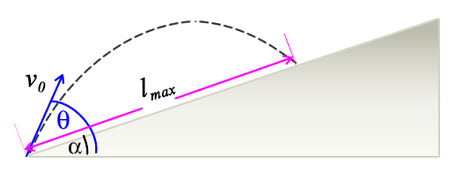
\includegraphics[scale=0.65]{Graphics/finalexam_p1}
\end{center}

``A gunman standing on a sloping ground fires up the slope. The initial speed of the bullet is $v_0 = 370$ m/s. The slope has an angle $\alpha = \ang{23}$ from the horizontal, and the gun points at an angle $\theta$ from the horizontal. The gravitational acceleration is $g = \SI{10}{m/s^2}$.

(a) For what value of $\theta$ ( where $\theta>\alpha$) does the gun have a maximal range along the slope? (In degrees, from the horizontal.)\\
(b) What is the maximal range of the gun, $\ell_{max}$, along the slope? (In meters.)''

Let's see. We want to maximize $\ell_{max}$, and also find the value of $\theta$ which causes it to be maximized. That is, we find a function $\ell_{max}(\theta)$, take its derivative, set that equal to zero, and look at the point(s) to find the maximum.

$\ell_{max}$ is not the total distance the bullet moves, of course; the parabolic trajectory is much longer than the actual distance moved along the slope. In order to find the diagonal distance, we can write down the $x$ and $y$ coordinates where the bullet hits, and use some trigonometry.

We can decompose the bullet's motion into $x$ and $y$ components. Using some simple trigonometry,

\begin{align}
\sin \alpha &= \frac{y}{\ell_{max}}\\
\cos \alpha &= \frac{x}{\ell_{max}}
\end{align}

So the coordinates where it lands are given by

\begin{align}
x &= \ell_{max} \cos \alpha\\
y &= \ell_{max} \sin \alpha
\end{align}

assuming the sensible choice of coordinate system, i.e. $x$ positive rightwards, $y$ positive upwards and the origin where the gunman is standing.

$v_0$ is at an angle $\theta$ to the ground; the components are given by

\begin{align}
v_{0x} &= v_0 \cos \theta\\
v_{0y} &= v_0 \sin \theta
\end{align}

The bullet coordinates as a function of time are, using $x(t) = x_0 + v_0 t + \frac{1}{2} a t^2$ where $a$ is constant,

\begin{align}
x(t) &= v_0 \cos (\theta) t\\
v_x(t) &= v_0 \cos \theta\\
y(t) &= v_0 \sin (\theta) t - \frac{1}{2} g t^2\\
v_y(t) &= v_0 \sin \theta - g t
\end{align}

The height at which it hits, as a function of $x$ (more simple trigonometry) is

\begin{equation}
y = x \tan \alpha
\end{equation}

We can then write that, at the point/time of collision,

\begin{align}
v_0 \cos (\theta) t &= x\\
v_0 \sin (\theta) t - \frac{1}{2} g t^2 &= x \tan \alpha
\end{align}

$x$, $\theta$ and $t$ are all unknown. We can substitute using $x = \ell_{max} \cos \alpha$, so that we have

\begin{align}
v_0 \cos (\theta) t &= \ell_{max} \cos \alpha\\
v_0 \sin (\theta) t - \frac{1}{2} g t^2 &= \ell_{max} \cos \alpha \tan \alpha
\end{align}

That doesn't change the number of unknowns, but it does get rid of the $x$. We can eliminate the time from the second equation by using the first,

\begin{equation}
t = \frac{\ell_{max} \cos \alpha}{v_0 \cos \theta}
\end{equation}

Substituting that in and simplifying,

\begin{align}
v_0 \sin (\theta) \left(\frac{\ell_{max} \cos \alpha}{v_0 \cos \theta}\right) - \frac{1}{2} g \left(\frac{\ell_{max} \cos \alpha}{v_0 \cos \theta}\right)^2 &= \ell_{max} \cos \alpha \tan \alpha\\
\ell_{max} \cos \alpha \tan \theta - \frac{1}{2} g \frac{\ell_{max}^2 \cos^2 \alpha}{v_0^2 \cos^2 \theta} &= \ell_{max} \cos \alpha \tan \alpha\\
\tan \theta - \frac{1}{2} g \frac{\ell_{max} \cos \alpha}{v_0^2 \cos^2 \theta} &= \tan \alpha
\end{align}

We can then solve for $\ell_{max}$.

\begin{align}
\ell_{max}(\theta) &= \frac{2 v_0^2 \cos^2 \theta}{g \cos \alpha} \left(\tan \theta - \tan \alpha\right)\\
\ell_{max}(\theta) &= \frac{2 v_0^2}{g \cos \alpha} \left(\cos^2 \theta \tan \theta - \cos^2 \theta \tan \alpha\right)
\end{align}

Our goal is now to maximize this. $v_0$ is a constant, $g$ is a constant and $\alpha$ is a constant. What we really want to maximize is therefore simply (well, it's not that simple, but still) this expression:

\begin{equation}
\cos^2 \theta \tan \theta - \cos^2 \theta \tan \alpha
\end{equation}

i.e. the expression in parenthesis. $\tan \alpha$ is a constant, which also helps.\\
By far the easiest way to do this is to graph that, and read off the answer, by the way! I did that to verify, but will try to carry out the full calculation.\\
We calculate the derivative of this with respect to $\theta$ and set that equal to zero, to find the maxima:

Part one:

\begin{equation}
\frac{d}{d\theta} \left(\cos^2 \theta \tan \theta\right) = \cos^2\theta \sec^2 \theta + \tan \theta ( -2 \sin\theta \cos \theta)
\end{equation}

Part two:
\begin{equation}
\frac{d}{d\theta} \left(\cos^2 \theta \tan \alpha\right) = -2 \sin \theta \cos \theta \tan \alpha
\end{equation}

So all in all,

\begin{align}
\cos^2\theta \sec^2 \theta + \tan \theta ( -2 \sin\theta \cos \theta) + 2 \sin \theta \cos \theta \tan \alpha\\
1 - 2\sin^2 \theta + 2 \sin \theta \cos \theta \tan \alpha
\end{align}

$\sec \theta = \frac{1}{\cos \theta}$, so those cancel. $\tan \theta = \frac{\sin\theta}{\cos\theta}$, so $\tan \theta \sin \theta \cos \theta = \sin^2\theta$.

This is still not pretty, but let's try. We set this equal to zero and try to solve for $\theta$:

\begin{align}
1 - 2\sin^2 \theta + 2 \sin \theta \cos \theta \tan \alpha &= 0\\
1 - 2\sin^2 \theta + \sin(2\theta) \tan \alpha &= 0\\
2\sin^2 \theta - \sin(2\theta) \tan \alpha &= 1
\end{align}

This is where I gave up and used Mathematica; these more hairy trig expressions aren't my favorite. This can apparently be simplified down to 

\begin{equation}
\cos (\alpha - 2 \theta) = 0
\end{equation}

which is easier to work with. Take the arccosine of both sides, and

\begin{align}
\alpha - 2 \theta &= -\frac{\pi}{2}\\
\alpha + \frac{\pi}{2} &= 2 \theta\\
\frac{\alpha}{2} + \frac{\pi}{4} &= \theta\\
\end{align}

OK, so I cheated a bit here; I first tried $\arccos(0) = \pi/2$, which gave me a negative angle for $\theta$, and so I tried a different choice. Choosing $-\pi/2$ instead gives a value for $\theta$ in the only possible range, $0 < \theta < \pi/2$.

This gives us $\theta \approx 0.98611$ radians, or 56.5 degrees. Plugging this value back into $\ell_{max}$, we find $\ell_{max} = 9843.74$ meters.

This answer looks unreasonably large to me, especially given the travel time with gravity in mind, but it does seem sensible if we compare it to a formula from lecture. The maximum horizontal distance it could travel (if the ground was flat) is $v_0^2 \sin(2\theta) / g$ meters, which evaluates to about 12600 m.\\
If this answer is correct, what are the coordinates where it hits? Using the formulas we found, it is about $x = 9061$ m and $y = 3846$ m(!).

The maximum height the bullet could reach is $(v_0 \sin \theta)^2 / (2g) \approx 4760$ meters, so this answer could be correct... and it is!

Well, that was a pain. This is one of those questions where I pretty much expect that there is a simpler solution. Granted, if I'd used Mathematica the entire way it wouldn't have been that hard, but surely that shouldn't be necessary.

\section{Problem 2: Angular collision}

\begin{center}
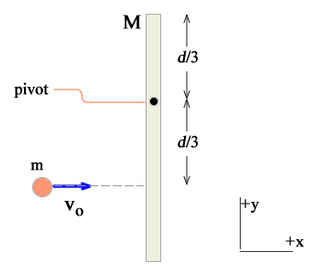
\includegraphics[scale=0.65]{Graphics/finalexam_p2}
\end{center}

``A uniform rod of mass $M$ and length $d$ is initially at rest on a horizontal and frictionless table contained in the xy plane, the plane of the screen. The figure is a top view, gravity points into the screen. The rod is free to rotate about an axis perpendicular to the plane and passing through the pivot point at a distance $d/3$ measured from one of its ends as shown. A small point mass $m$, moving with speed $v_0$, hits the rod and stick to it at the point of impact at a distance $d/3$ from the pivot.

(a) If the mass of the rod is $M=4m$, what is the magnitude of the angular velocity of the rod+small mass system after the collision?''

\begin{enumerate}
\item $\omega = 2 v_0/(3 d)$
\item $\omega = 3 v_0/(2 d)$
\item $\omega = 4 v_0/(3 d)$
\item $\omega = 3 v_0/(4 d)$
\item $\omega = 8 v_0/(3 d)$
\item $\omega = 3 v_0/(8 d)$
\item $\omega = 5 v_0/(3 d)$
\item $\omega = 3 v_0/(5 d)$
\end{enumerate}

My first try was way incorrect -- I misread the question completely. I read it as a collision a distance $d/3$ from the center of mass, and didn't even realize it wasn't completely free to move. Geez -- reading carefully is important, and I should know better than to \emph{not} read very carefully.

So there's a pivot point, which is located a distance $d/3$ from the \emph{end} of the rod. The end is located a distance $d/2$ from the center of the rod, and so the pivot point is located $d/2 - d/3 = d/6$ from the rod's center (of mass).

We can use the relationship $L = I \omega$ to find $\omega$. The angular momentum of the rod prior to the collision is zero, so the angular impulse from the collision will equal its final angular momentum $L$, about the pivot point.\\
What is the moment of inertia $I$ about this point though? We start off with the moment of inertia of a rod, about its center of mass, which is $\frac{1}{12} M d^2$. Next, we need to increase that by an amount $M (d/6)^2$ via the parallel axis theorem, as we aren't rotating it about its center of mass.\\
Finally, we must add the moment of inertia due to the point mass, which is $m r^2$, where $r$ is the distance between the rotation axis and the point where it is stuck. ($r$ is \emph{not} the distance from the center of mass to that point -- if it were stuck at the rod's center of mass, it would still have a nonzero contribution!)\\
That distance is $r = d/3$ as given in the problem, so we add $m r^2 = m (d/3)^2 = \frac{1}{9} m d^2$, for a total moment of inertia of

\begin{equation}
I = I_{cm,rod} + I_{parallelaxis} + I_{pointmass} = \frac{1}{12} M d^2 + \frac{1}{36} M d^2 + \frac{1}{9} m d^2
\end{equation}

Using $M = 4m$, this simplifies to

\begin{equation}
I = \frac{1}{3} m d^2 + \frac{1}{9} m d^2 + \frac{1}{9} m d^2 = \frac{5}{9} m d^2
\end{equation}

Next, what is the angular impulse about the pivot point? The linear impulse is simply $m v_0$; to find the angular impulse, we multiply this by the distance between the impact point and the pivot point, $d/3$. As mentioned previously, the post-collision angular momentum will be equal to this angular impulse, so:

\begin{equation}
\omega = \frac{L}{I} = \frac{ \frac{m v_0 d}{3} }{\frac{5}{9} m d^2} = \frac{9m v_0 d}{15 m d^2} = \frac{3 v_0}{5 d}
\end{equation}

``(b) Using again $M=4m$. What is the speed of the center of mass of the rod right after collision?''

\begin{enumerate}
\item $v_{cm} = v_0$
\item $v_{cm} = v_0/2$
\item $v_{cm} = v_0/3$
\item $v_{cm} = v_0/5$
\item $v_{cm} = v_0/10$
\item $v_{cm} = v_0/20$
\end{enumerate}

We can simply use $v = \omega R$, where $R$ is the distance between the pivot point and the point we care about, i.e. the center of mass. We said earlier that this distance was $d/6$, so

\begin{equation}
v_{cm} = \frac{3 v_0}{5 d} \times \frac{d}{6} = \frac{v_0}{10}
\end{equation}

\section{Problem 3: Atmospheric pressure}

``In the lecture, we discussed the case of an isothermal atmosphere where the temperature is assumed to be constant. In reality, however, the temperature in the Earth's atmosphere is not uniform and can vary strongly and in a non-linear way, especially at high altitude. To a good approximation, the temperature $T$ drops almost linearly with altitude up to 11 km above sea level, at a constant rate:

\begin{equation}
\frac{dT}{dz} = -\alpha \text{ for } z \le 11 \text{ km}
\end{equation}

where $\alpha = 6.5$ K/km (Kelvin per km) and $z$ is the height above the sea level. The temperature stays then approximately constant between 11 km and 20 km above sea level.

Assume a temperature of $15{}^\circ$C and a pressure of 1 atm at sea level (1 atm = $\SI{1.01325e5}{N/m^2}$). Furthermore, take the molecular weight of the air to be (approximately) 29 g/mol. The universal gas constant is $R = \SI{8.314}{J K^{-1} mol^{-1}}$ and the acceleration due to gravity is $g = \SI{10}{m/s^2}$ (independent of altitude). Assume that air can be treated as an ideal gas.

(a) Under the assumptions above, calculate the atmospheric pressure $p$ (in atm) at $z = 10$ km above sea level for the case of a linear temperature drop.''

Let's see! In lecture, for calculating this in the case of an isothermal atmosphere, we calculated the density as

\begin{equation}
\rho = \frac{N m}{V}
\end{equation}

where $N$ is the number of molecules, $m$ the mass (in kg) of each molecule, $V$ the volume and $\rho$ the density of that (small) volume. We also used the ideal gas law in the form $P V = N k T$, as we also will here. We rearrange it a bit

\begin{equation}
\frac{P}{kT} = \frac{N}{V}
\end{equation}

Using $\rho = \frac{N m}{V}$, we substitute a bit to find

\begin{equation}
\rho=\frac{P m}{k T(z)}
\end{equation}

Still as in lecture, but with the important change I noted just above, that the temperature is now a function of $z$.\\
We we substitute this into the separable differential equation that we previously used to derive Pascal's law:

\begin{equation}
\frac{dP}{dz} = - \rho(z) g = - \frac{P mg}{k T(z)}
\end{equation}

We rearrange this,

\begin{equation}
\frac{\mathop{dP}}{P} = - \frac{mg}{k T(z)} \mathop{dz}
\end{equation}

This is where things change. We now need to consider T(z), where $T'(z) = -\alpha$ up to 11 km, and then zero ($T(z) = \text{constant}$) up to 20 km.

Since the temperatures is 15 degrees C at sea level, and it drops by 6.5 K/km, the temperature at 11 km to 20 km must be -56.5 C. In between, the temperature is $15 - \alpha z = 15 - 6.5 z$ degrees C. The problem only asks about stuff up to 10 km, however, and what happens above is of little concern to us; it doesn't enter into the equations.

We need to convert the temperature to kelvin, which we do by adding 273.15 to the number. I also find it more sensible to work in terms of meters, not kilometers. Therefore, $\alpha = \SI{6.5e-3}{K/m}$, and

\begin{equation}
T(z) = 288.15 - (\SI{6.5e-3}{K/m}) z
\end{equation}

which is valid up to 11 000 m.

Moving on, we substitute this into our equation:

\begin{equation}
\frac{\mathop{dP}}{P} = - \frac{mg}{k (288.15 - (\SI{6.5e-3}{K/m}) z)} \mathop{dz}
\end{equation}

Or, in terms of symbols where $T_0$ is the temperature at sea level,

\begin{equation}
\frac{\mathop{dP}}{P} = - \frac{mg}{k (T_0 - \alpha z)} \mathop{dz} = C \frac{1}{T_0 - \alpha z} \mathop{dz}
\end{equation}

where $C = -\frac{m g}{k}$.

I prefer this form for the integration, since the constants and units look messy. For the first time, I chose to use the rather quaint method of a lookup table. I found

\begin{equation}
\int \frac{1}{a x + b} \mathop{dx} = \frac{1}{a} \ln (|ax + b|)
\end{equation}

Since $C$ is a constant, we can move that outside the integral. We then just map $a = -\alpha$ and $b = T_0$, so the result is

\begin{align}
C \frac{1}{a} \ln (|ax + b|) &= -\frac{C}{\alpha} \ln (|T_0 - \alpha z|)\\
                                     &= \frac{m g}{k \alpha} \ln (|T_0 - \alpha z|)
\end{align}

So we can finally go to calculate the definite integrals. The left-hand side is easy (and unchanged since lecture). On the right-hand side, we do what we did above, and substitute for $h$ and $0$:

\begin{align}
\frac{\mathop{dP}}{P} &= - \frac{mg}{k (T_0 - \alpha z)} \mathop{dz}\\
\int_{P_0}^{P_h} \frac{\mathop{dP}}{P} &= - \frac{mg}{k} \int_0^h \frac{1}{T_0 - \alpha z} \mathop{dz}\\
\ln P_h - \ln P_0 &= \frac{m g}{k \alpha} \ln (|T_0 - \alpha h|) - \frac{m g}{k \alpha} \ln (T_0)\\
\ln \frac{P_h}{P_0} &= \frac{m g}{k \alpha} \left( \ln (T_0 - \alpha h) - \ln (T_0)\right)\\
\ln \frac{P_h}{P_0} &= \frac{m g}{k \alpha} \ln (1 - \frac{\alpha h}{T_0})
\end{align}

I removed the absolute value bars since $T_0 > \alpha h$ for all values that we use.

We can now exponentiate both sides of this equation.

\begin{align}
\frac{P_h}{P_0} &= e^{\frac{m g}{k \alpha} \ln (1 - \frac{\alpha h}{T_0})}\\
P_h &= P_0 e^{\frac{m g}{k \alpha} \ln (1 - \frac{\alpha h}{T_0})}
\end{align}

This should be a useful answer, but we can manipulate it a bit further, using $e^{a \ln b} = b^a$, so that

\begin{equation}
P_h = P_0 \left(1 - \frac{\alpha h}{T_0}\right)^{\dfrac{m g}{k \alpha}}
\end{equation}

Plotting this versus the lecture's $P_h = P_0 e^{-h/H_0}$ with $H_0 = 8000$ m, it's clear that the two are very similar. For heights less than 1 km, they are \emph{very similar} (hard to see a difference at all on a plot). At 10 km, where the error is the greatest, the difference is still only some 10-14\%.

Finally, to answer question (a): using this formula, the pressure at $z = 10$ km, using $P_0 = 1$ atm, the pressure is $P_h = 0.253613$ atm. For comparison, the lecture's equation gives $P_h = 0.286505$ atm, about 13\% more.

To find the answer, I used $\alpha = \SI{6.5e-3}{K/m}$, $T_0 = \SI{288.15}{K}$, $m = 29 \times \SI{1.66e-27}{kg}$, $g = \SI{10}{m/s^2}$ and $k = R/N_A \approx \SI{1.38e-23}{J/K}$.

``(b) The cruising altitude of a commercial aircraft is about 33'000 ft (or 10 km). Assume that the cabin is pressurized to 0.8 atm at cruising altitude. What is the minimal force Fmin (in Newton) per square meter that the walls have to sustain for the cabin not to burst? Use the atmospheric pressure found in (a).''

Well, this is certainly easy compared to all the above!\\
The internal pressure is 0.8 atm, but the external pressure only 0.2536 atm. The pressure difference is what gives rise to the force on the walls, and that difference is 0.5464 atm, or 55362.7 pascal (newton per square meter), which answers this question.

``(c) We close a plastic bottle full of air inside the cabin when the aircraft is at cruising altitude of $z = 10$ km. The volume of the bottle is $V_1$, the pressure and temperature inside the cabin are 0.8 atm and $T_1 = \SI{27}{\degreeCelsius}$, respectively. Assume that at sea level the atmospheric pressure is 1 atm, and the temperature is decreased by 10 Kelvin with respect to the cabin's temperature.

What is the magnitude of the percentage change in volume of the air inside the bottle when it is brought to sea level? Enter the magnitude of the percentage change in volume in

\begin{equation}
\Big| \frac{\Delta V}{V_1} \Big| \times 100
\end{equation}

OK. We begin with a certain volume, and then increase the pressure and decrease the temperature. Using the ideal gas law, the volume for the two cases is

\begin{align}
V_1 &= \frac{n R T_1}{P_1}\\
V_2 &= \frac{n R T_2}{P_2}
\end{align}

$\Delta V = V_2 - V_1$, so

\begin{equation}
\Big| \frac{\Delta V}{V_1} \Big| \times 100 = \Big| \frac{V_2}{V_1} - 1\Big| \times 100 = \Big| \frac{P_1 T_2}{P_2 T_1} - 1\Big| \times 100
\end{equation}

We substitute in $P_1 = 0.8$ atm, $P_2 = 1$ atm, $T_1 = 300.15$ K and $T_2 = 290.15$ K and find an answer of $22.6\%$.

\section{Problem 4: Prisms}

\begin{center}
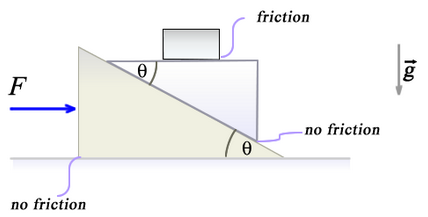
\includegraphics[scale=0.65]{Graphics/finalexam_p4}
\end{center}

``In the diagram, both the prisms and the block have equal masses $m$. Angle $\theta$ is given. Both surfaces of the larger prism are frictionless; however, there is friction between the horizontal surface of the smaller prism and the block. A horizontal and constant force of unknown magnitude F is exerted on the larger prism. As a result, the three objects remain at rest relative to each other.

(a) Find the magnitude of the acceleration of the larger prism a.''

\begin{enumerate}
\item $a = 2 g \tan \theta$
\item $a = g \tan \theta$
\item $a = g \sin \theta$
\item $a = 2 g \cos \theta$
\item $a = g \cos \theta$
\item $a = 2g \sin \theta$
\end{enumerate}

''(b) Find the value of the pushing force F.''

\begin{enumerate}
\item $F = 6 m g \tan \theta$
\item $F = 6 m g \sin \theta$
\item $F = 6 m g \cos \theta$
\item $F = 3 m g \cos \theta$
\item $F = 3 m g \sin \theta$
\item $F = 3 m g \tan \theta$
\end{enumerate}

''(c) Find the minimum coefficient of static friction $\mu_s$ between the block and the smaller prism that makes it possible for the block to stay at rest relative to the prism.''

\begin{enumerate}
\item $\mu_s = 2 \tan \theta$
\item $\mu_s = \tan \theta$
\item $\mu_s = 2 \sin \theta$
\item $\mu_s = \sin \theta$
\item $\mu_s = 2 \cos \theta$
\item $\mu_s = \cos \theta$
\end{enumerate}

OK. So this problem is a slightly strange one, I think; when I just glanced over it as I copied it down, I figured the system was standing still, and the force was on the ``middle prism''; turns out the force is on the leftmost prism instead, so that the entire thing must be constantly accelerating, sliding faster and faster, for this to work!

If $F = 0$, the lower prism would glide towards the left, while the upper prism would glide down and towards the right.

$a$ for one object must be the same for all three, since they are at rest relative to each other.\\
The total mass of the three objects is $3m$, and since $F$ in the only horizontal external force, $a = F/(3m)$ must hold.

My first take on this one was incorrect -- the answer I found wasn't among the options, so I didn't waste any submissions, however.\\
I noticed that if I wrote the normal force in terms of $\sec\theta$ instead of $\cos\theta$, the answer was listed, though I couldn't really figure out \emph{why} that would be correct. I did come up with the solution after a while, and got it right. A few hours later, I came up with this simpler solution, which stared me in the face the entire time. (I had tried to find an equation that I'd basically already written down, only rearranged.)

Anyway, let's look at the forces involved. On the top block, there are three forces: gravity at $m g$ straight down, a normal force of that same magnitude straight up, and a frictional force $\mu_s m g$, towards the right. (This is the force that provides the acceleration of the block.)\\
This is, by the way, using the condition that the block is about to slip; $F_f \le \mu_s m g$ in general, but in the about-to-slip case, it is exactly equal.

On the top prism (or middle, if you prefer), the weight of the top block is acting downwards with magnitude $m g$, and the weight of the prism itself too, for a total downward force $2 m g$. Then there's a force $\mu_s m g$ towards the \emph{left} -- the Newton's third law pair of the friction acting on the block.\\
Finally, there's the normal force from the bottom prism, acting diagonally upwards. The horizontal component of this, $N \sin \theta$ is the source of acceleration for this prism. The vertical component must be $N \cos \theta = 2 m g$, or there would be vertical acceleration of the prism.

As for the bottom prism, we can restrict ourselves to horizontal forces. That leaves $F$, the source of the acceleration, and $N$ acting diagonally downwards/towards the left. The horizontal component of magnitude $N \sin \theta$ opposes the motion.

All in all, this gives us a bunch of equations:

\begin{align}
F - N \sin \theta &= m a &&\text{ Newton's second law, bottom prism}\\
N \sin \theta - \mu_s m g &= m a &&\text{ Newton's second law (horizontal), top prism}\\
N \cos \theta &= 2 m g &&\text{ Newton's second law (vertical), top prism}\\
\mu_s m g &= m a &&\text{ Newton's second law, block}
\end{align}

Note that I use $N$ to denote the normal force acting on the top prism; there are several other normal forces, but they aren't as important. Via Newton's third law, this force also acts on the bottom prism.

From the last equation, we have $\mu_s = a/g$ -- that should be very helpful once we have $a$.\\
If we rewrite the $N \sin \theta - \dots$ equation using this relationship for $\mu_s$, we get $N \sin \theta = 2 ma$. We can then divide that by the equation right below, and get

\begin{align}
\tan \theta &= \frac{2 ma}{2 m g}\\
g \tan \theta &= a
\end{align}

Excellent! We then know $a$, and also $\mu_s = a/g = \tan \theta$. Only $F$ remains. Now, the easy way is to use $F/(3m) = a$ as I mentioned earlier, but we can use these equations as well. From the first equation in the group above, using the now-known value for $a$ and that of $N \sin \theta = 2 m a$,

\begin{align}
F - N \sin \theta &= m a\\
F - 2 m a &= m a\\
F &= 3 m a\\
F &= 3 m g \tan \theta
\end{align}

And we are done! To summarize, the answers are

\begin{align}
a &= g \tan \theta\\
F &= 3 m g \tan \theta\\
\mu_s &= \tan \theta
\end{align}

\section{Problem 5: A harmonic oscillator}

\begin{center}
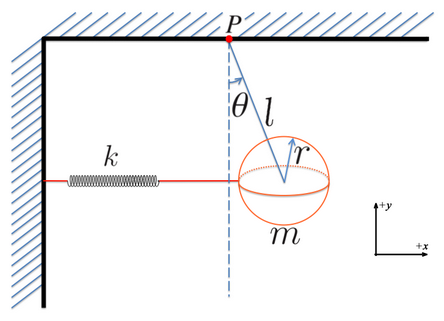
\includegraphics[scale=0.65]{Graphics/finalexam_p5}
\end{center}

``A pendulum of mass $m = 0.9$  kg and length $\ell = 1$ m is hanging from the ceiling. The massless string of the pendulum is attached at point P. The bob of the pendulum is a uniform shell (very thin hollow sphere) of radius $r = 0.4$ m, and the length $\ell$ of the pendulum is measured from the center of the bob. A spring with spring constant $k = \SI{10}{N/m}$ is attached to the bob (center). The spring is relaxed when the bob is at its lowest point ($\theta = 0$). In this problem, we can use the small-angle approximation $\sin \theta \approx \theta$ and $\cos \theta \approx 1$. Note that the direction of the spring force on the pendulum is horizontal to a very good approximation for small angles $\theta$. (See figure)\\
Take $g = \SI{10}{m/s^2}$.

(a) Calculate the magnitude of the net torque on the pendulum with respect to the point P when $\theta = \ang{5}$. (magnitude; in Nm)\\
(b) What is the magnitude of the angular acceleration $\alpha = \ddot{\theta}$ of the pendulum when $\theta = \ang{5}$? (magnitude; in $\text{radians/s}^2$)\\
(c) What is the period of oscillation $T$ of the pendulum? (in seconds)''

First of all, let's not forget that the moment of inertia of a spherical shell is \emph{not} $\frac{2}{5} m r^2$ -- that holds for solid spheres only! The relevant moment of inertia is $\frac{2}{3} m r^2$.

With that in mind, lets try to analyze the situation. I started by drawing it all out.\\
The torque on the bob is given by the torque due to gravity, $\vec{\ell} \times \vec{F_g}$ plus the torque due to the spring, $\vec{\ell} \times \vec{F_{spr}}$.\\
The former is $\ell m g \sin \theta$; $\sin \theta$ because of the cross product, while there other terms should be rather clear.

So what is the torque due to the spring force? Well, first, what \emph{is} the spring force? It's clear that it will be leftwards at this moment, just as the torque due to gravity.
The magnitude is simply $k$ times the extension of the spring. Since it is at equilibrium when $\theta = 0$, it is stretched an amount $\ell \sin \theta$ past that.\\
To find the torque, we take $\ell$ (the lever arm; there is no torque relative to the bob's center since the spring is fastened there, but there is a torque relative to point P) and multiply that by the spring force $k \ell \sin \theta$.\\
We should then multiply this by the sine of the angle between the two vectors; that angle is $\theta + \ang{90}$, which gives us a $\cos \theta$ term via $\sin(\ang{90} + \theta) = \cos \theta$. We can approximate this term as 1 and ignore it, since we are allowed to use the small angle approximation.

We then know the torque relative to point P, which is

\begin{equation}
\tau_P = \ell m g \sin \theta + k \ell^2 \sin \theta
\end{equation}

We apply the small angle approximation to the sine terms as well, and find

\begin{equation}
\tau_P = \ell m g \theta + k \ell^2 \theta
\end{equation}

Next, we calculate the moment of inertia of the bob. About its center of mass, it is simply $\frac{2}{3} m r^2$ (moment of inertia for a hollow sphere/thin spherical shell), but we want the moment of inertia about point P. We must therefore add a term $m \ell^2$ via the parallel axis theorem. The total moment of inertia about point P is

\begin{equation}
I_P = \frac{2}{3} m r^2 + m \ell^2
\end{equation}

Finally, we use the relationship $\tau = -I \alpha$ (not forgetting the minus sign for the restoring torque) to find $\alpha$ as the ratio of these two quantities (I also wrote $\alpha$ as $\ddot{\theta}$):

\begin{equation}
\ddot{\theta} = - \frac{\ell m g + k \ell^2}{\frac{2}{3} m r^2 + m \ell^2} \theta
\end{equation}

(Without the minus sign, this equation would not make sense: it would state that as you move the bob towards the right, the angular acceleration would grow in that same direction.)

This is in the form $\ddot{\theta} = -\omega^2 \theta$ (with $\omega$ being a constant), which is a simple harmonic oscillation. We can calculate the answer to part (b) using the above equation, and then use the solution to the above differential equation to find the period, part (c).

The period is given by $\displaystyle T = \frac{2\pi}{\omega}$, where $\omega$ is (as noted above) the square root of the term multiplying $\theta$.

\begin{align}
\omega &= \sqrt{\frac{\ell m g + k \ell^2}{\frac{2}{3} m r^2 + m \ell^2}}\\
T &= 2 \pi \sqrt{\frac{\frac{2}{3} m r^2 + m \ell^2}{\ell m g + k \ell^2}}
\end{align}

We then have the answers to all the questions. The magnitude of the torque is easily calculated as $1.656$ newton-meters using the equation above; I used the one \emph{without} the small angle approximation, but they are very close together.

Next, $\alpha = \ddot{\theta}$ is also rather easy to calculate using the equation we have for that (with the small angle approximation). There, I find $|\ddot{\theta}|$ as $\SI{1.665}{rad/s^2}$. Finally, the period is calculated as $1.439$ seconds.

\section{Problem 6: Gliding mass stopped by spring}

``A small block of mass $m = 1$ kg glides down (without friction) a circular track of radius $R = 2$ m, starting from rest at height $R$. At the bottom of the track it hits a massless relaxed spring with spring constant $k = 7$ N/m, which starts to be compressed as the block continues to move horizontally. Note that we assume no energy loss during this 'collision'. There is friction between the block and the horizontal surface, and it is not uniform. As a function of distance, the friction coefficient varies like $\mu(x)=\alpha x$, with $\alpha= 0.6  \text{m}^{-1}$. Assume for simplicity that static and dynamic friction coefficients are the same, and use $g = \SI{10}{m/s^2}$. (See figure)

\begin{center}
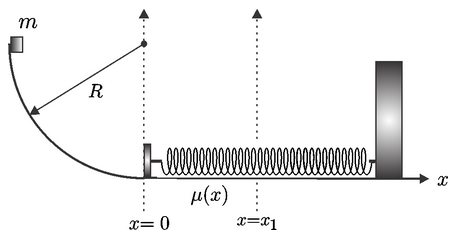
\includegraphics[scale=0.65]{Graphics/finalexam_p6}
\end{center}

(a) What is the maximal distance $x_1$ that the block moves horizontally away from the track at $x = 0$? (in meters)\\
(b) What time $t_1$ does it take for the block to travel between $x = 0$ (relaxed spring) and $x = x_1$ (block at first stop)? (in seconds)\\
(c) What will happen after the block reaches point $x_1$?''

\begin{enumerate}
\item The block will move back and get catapulted up the circular track.
\item The block will move back and reach a second stop somewhere between $x = 0$ and $x = x_1$.
\item The block will move back and reach a second stop exactly at $x = 0$.
\item The block will stay put forever at $x = x_1$
\end{enumerate}

All right, this looks like an interesting problem.\\
With no frictional losses on the circular track, we can use conservation of energy to calculate its ``initial'' velocity (at the ``collision''). If we take the horizontal surface as $y = 0$ and $U = 0$, the initial gravitational potential energy is $m g R$, and the initial kinetic energy 0. The sum of the two must equal the kinetic energy as it exits the circular track, plus the gravitational potential energy at that point, which we defined as zero.

\begin{align}
\frac{1}{2} m v^2 &= m g R\\
v &= \sqrt{2 g R}
\end{align}

Once it reaches the horizontal surface, we have two forces opposing our motion: the spring force of magnitude $k x$, and the frictional force of magnitude $F_f = \mu_s m g = \alpha x m g$. This causes a leftwards acceleration (i.e. our velocity decreases) of

\begin{equation}
a = \frac{\sum |}{m} = -\frac{k + \alpha m g}{m} x
\end{equation}

At first, I didn't write it down like this, and so I didn't realize that this is a  simple harmonic oscillation! ($a = \ddot{x}$.)\\
We have friction, but other than that, it should be rather clear.\\
I first wanted to solve it in terms of integration acceleration, but the force is a function of $x$, which makes that harder. Next, I considered an energy analysis (or power, rather) where I had similar problems. Let's look at simple harmonic motion instead. Above, we have

\begin{equation}
\ddot{x} = -\frac{k + \alpha m g}{m} x
\end{equation}

This equation is clearly not always valid; the oscillation will die out. We can use this for the ``compression phase'', though, i.e. until the mass stops. The solution is

\begin{align}
x &= x_1 \cos (\omega t + \varphi)\\
\dot{x} &= -x_1 \omega \sin(\omega t + \varphi)\\
\omega &= \sqrt{\frac{k + \alpha m g}{m}}\\
T &= \frac{2 \pi}{\omega} = 2\pi \sqrt{\frac{m}{k + \alpha m g}}
\end{align}

I was about to write $x_{max}$ for the amplitude, but the amplitude is what we call $x_1$ in this problem.\\
We need to use $\dot{x}$ to find the ``amplitude'' $x_1$ and the phase angle $\varphi$. We should be able to calculate the time taken (part b) as $T/4$, but let's take one step at a time.

By setting the $x$ and $\dot{x}$ equations to their respective values at $t = 0$ (our initial conditions), we find

\begin{align}
0 &= x_1 \cos (\varphi)\\
\sqrt{2 g R} &= - x_1 \sqrt{\frac{k + \alpha m g}{m}} \sin (\varphi)
\end{align}

The first equation must imply that $\varphi = \pi/2$ or $\varphi = 3\pi/2$, since $x_1 \neq 0$. If that's the case, the sine term in the second equation becomes $1$, and so

\begin{align}
\sqrt{2 g R} &= - x_1 \sqrt{\frac{k + \alpha m g}{m}}\\
x_1 &= -\sqrt{2 g R} \frac{1}{\sqrt{\frac{k + \alpha m g}{m}}}
\end{align}

This has a sign error, so the phase must be $3 \pi/2$ so that the sine is $-1$ and $x_1$ is positive.

\begin{align}
x_1 &= \frac{\sqrt{2 m g R}}{\sqrt{k + \alpha m g}}
\end{align}

This gives us $x_1 = 1.754$ meters.\\
Via the period formula, $T = 1.74264$ seconds, though we are interested in a quarter of that value, $T/4 = 0.43566$ seconds.\\
(In the first quarter, the mass moves from $x=0$ to $x = x_1$. In the second, it moves back. In the third, it moves to $x = -x_1$, and in the fourth, it moves back to $x = 0$. Assuming no friction, that is; in this case, things will change.)

What happens next? Well, the maximum static friction at this location is $\mu_s m g = \alpha x m g = 10.52$ N. The spring force is $k x = 12.278$ N, so static friction will be overcome, and the system will start to move. That leaves options 1, 2 and 3.

The spring has a stored energy of $\frac{1}{2} k x^2 = 10.77$ J, compared to the initial kinetic energy $\frac{1}{2} m v^2 = m g R = 20$ J. Just less than half the energy was wasted due to friction as the block came to a temporary halt. Does this make it safe to assume it will move past $x = 0$ again, though? In terms of energy, I'm not sure.\\
However, the spring force is always larger than the frictional force, as $k > \alpha m g$ (and so, of course, $k x > \alpha m g x$), meaning that not only can't it come to a halt prior to $x = 0$, it cannot \emph{slow down}, either; it will have a positive acceleration until it loses contact with the spring. Therefore it must be catapulted back up!

\section{Problem 7: Sliding blocks}

``A small cube of mass $m_1 = 1.0$ kg slides down a circular and frictionless track of radius $R = 0.4$ m cut into a large block of mass $m_2 = 4.0$ kg as shown in the figure below. The large block rests on a horizontal and frictionless table. The cube and the block are initially at rest, and the cube $m_1$ starts from the top of the path. Find the speed of the cube $v_1$ as it leaves the block. Take $g = \SI{10.0}{m/s^2}$. Enter your answer in m/s.''

\begin{center}
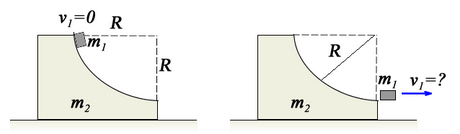
\includegraphics[scale=0.75]{Graphics/finalexam_p7}
\end{center}

All right. First, if the larger block was fastened to the table and did not move at all, the velocity could be found as $\sqrt{2 g R} \approx 2.8284$ m/s as in the previous problem. The answer we find here must be smaller, since some of the energy will go towards moving the bigger block in the opposite direction. In other words, the number above is an upper bound.

My solution was more complex than it needed to be, literally: when I reached the end, I had three equations with three unknowns. I solved the first equation for $N$, the normal force on the cube by the ramp, but realized that equation was the only one of the three to contain that term! That equation turned out to be useless, and the other two alone solved the problem. With that in mind, I cut out everything I wrote regarding forces and centripetal force. Instead, I used the conservation of mechanical energy and conservation of momentum alone.

First, we can write a conservation of energy equation. I will use $v_B$ for the velocity of the large block/ramp.

\begin{equation}
\frac{1}{2} m_1 v_1^2 + \frac{1}{2} m_2 v_B^2 = m_1 g R
\end{equation}

The total energy available at the start is $m_1 g R$, and since no energy is lost to e.g. friction, that must be a constant throughout.\\
$v_1$ and $v_B$ are both unknown, so we need a second equation. If we define it to be zero at the height where the cube flies off, 100\% of the initial energy has turned into kinetic energy at that point.

What more can we use? Well, we can also apply the conservation of momentum in the horizontal direction. Since the initial momentum of the block+cube system is zero, it must always be zero, since there are no external horizontal forces (e.g. friction between block and table).

\begin{equation}
m_1 v_1 - m_2 v_B = 0
\end{equation}

I wrote $m_2 v_B$ as negative, so that $v_B > 0$ while the momentum is towards the left.\\
We then have two equations and two unknowns -- very simple.

I'll start by solving the second one of these for $v_B$, which gives me $v_B = (m_1/m_2) v_1$.\\
We can substitute this into the larger equation, and solve for $v_1$.

\begin{align}
\frac{1}{2} m_1 v_1^2 + \frac{1}{2} m_2 \left(\frac{m_1}{m_2} v_1\right)^2 &= m_1 g R\\
\end{align}

I find $v_1 = 2.529$ m/s, about 90\% of what we would find if the ramp was immovable. The ramp itself is moving at $v_B = 0.632$ m/s towards the left (calculation not shown; I used Mathematica for that one as a quick test), with momentum $2.529$ kg m/s, as expected -- the cube's mass is exactly 1 kg, so its momentum has the same value as its velocity, as can be seen here; the two are identical in magnitude, but opposite in direction, so the total horizontal momentum is indeed zero.

That ends this exam, this course and these notes! Thanks for reading.

\end{document}
